\documentclass{tufte-handout}

\usepackage{amsmath}
\usepackage{amsthm} %needed for the proofs 
\usepackage{amssymb}
\usepackage{bm} %for bold math symbols
\usepackage{xcolor} %for heading colors
\usepackage{titling}
\usepackage{thmtools}
\usepackage[linesnumbered,ruled,vlined]{algorithm2e} %For pseudocode

%For plots
\usepackage{pgfplots}
\pgfplotsset{compat = newest}

%citations 

\newtheoremstyle{mytheoremstyle}
    {6pt} % space above
    {6pt} % space below
    {\normalfont} % body font
    {} % indent amount
    {\bfseries\color{blue}} % theorem head font
    {.} % punctuation after theorem head
    {1em} % space after theorem head
    {\thmname{#1}\thmnumber{ #2}\thmnote{ (#3)}} % theorem head spec

\newtheoremstyle{corlstyle}
    {6pt} % space above
    {6pt} % space below
    {\normalfont} % body font
    {} % indent amount
    {\textit{}} % theorem head font
    {.} % punctuation after theorem head
    {1em} % space after theorem head
    {\thmname{#1}\thmnumber{ #2}\thmnote{ (#3)}} % theorem head spec

% Define the theorem environment
\declaretheorem[style=mytheoremstyle,name=Theorem,numberwithin=section]{theorem}

% Define the corollary environment linked to the theorem
\declaretheorem[style=corlstyle,name=Corollary,numberlike=theorem,parent=theorem]{corollary}

\declaretheorem[style=corlstyle,name=Remark,numberlike=theorem]{remark}

\declaretheorem[style=corlstyle,name=Example,numberlike=theorem]{example}

% Define the lemma environment linked to the theorem
\declaretheorem[style=mytheoremstyle,name=Lemma,numberlike=theorem]{lemma}

% Define the proposition environment linked to the theorem
\declaretheorem[style=mytheoremstyle,name=Proposition,numberlike=theorem]{proposition}

% Define the definition environment linked to the theorem
\declaretheorem[style=mytheoremstyle,name=Definition,numberlike=theorem]{definition}

\newcommand\sol{%
  \\ 
  \\
  \textit{Solution:}\\%
}
\newcommand{\indep}{\perp \!\!\! \perp}

% Statistics operators
\DeclareMathOperator{\var}{Var}
\DeclareMathOperator{\cov}{Cov}

%Convex optimisation operators
\DeclareMathOperator{\cl}{cl}
\DeclareMathOperator{\epi}{epi}
\DeclareMathOperator{\lev}{lev}
\DeclareMathOperator{\dom}{dom}
\DeclareMathOperator{\aff}{aff}
\DeclareMathOperator{\ri}{ri}
\DeclareMathOperator{\argmin}{argmin}
\DeclareMathOperator{\argmax}{argmax}
\DeclareMathOperator{\R}{\mathbb{R}}
\DeclareMathOperator{\E}{\mathbb{E}}
\DeclareMathOperator{\inte}{int}
\DeclareMathOperator{\lin}{lin}
\DeclareMathOperator{\conv}{conv}
\DeclareMathOperator{\cont}{cont}
\DeclareMathOperator{\prox}{prox}
%\geometry{showframe} % display margins for debugging page layout

\usepackage{graphicx} % allow embedded images
  \setkeys{Gin}{width=\linewidth,totalheight=\textheight,keepaspectratio}
  \graphicspath{{graphics/}} % set of paths to search for images


\usepackage{booktabs} % book-quality tables
\usepackage{units}    % non-stacked fractions and better unit spacing
\usepackage{multicol} % multiple column layout facilities
\usepackage{lipsum}   % filler text
\usepackage{fancyvrb} % extended verbatim environments
\fvset{fontsize=\normalsize}% default font size for fancy-verbatim environments

% Prints a trailing space in a smart way.
\usepackage{xspace}

% Generates the index
%\usepackage{makeidx}
%\makeindex

\setcounter{secnumdepth}{4} %to set the section numbering


\newsavebox{\titleimage}
\savebox{\titleimage}{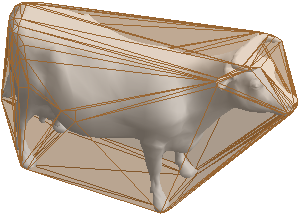
\includegraphics[height=15\baselineskip]{cvx_hull_cow.png}}

\makeatletter
\renewcommand{\maketitlepage}{%
\begingroup%
\setlength{\parindent}{0pt}

{\fontsize{18}{18}\selectfont\textit{\@author}\par}

\vspace{1.75in}{\fontsize{36}{54}\selectfont\@title\par}

\vspace{0.5in}{\fontsize{14}{14}\selectfont\textsf{\smallcaps{\@date}}\par}

\vspace{0.5in}\usebox{\titleimage}

\vfill{\fontsize{14}{14}\selectfont\textit{\@publisher}\par}

\thispagestyle{empty}
\endgroup
\newpage
}
\makeatother
% Book metadata
\title{MATH 563 Convex Optimization}
\date{\today}
\author{Alexandre St-Aubin}
\publisher{Taught by Courtney Paquette}

\begin{document}

\maketitlepage% this prints the handout title, author, and date

% r.5 contents
\tableofcontents
\newpage

\section{Chapter 1: Preliminaries}
\subsection{Euclidean Setting}%
  \label{sub:Eucledian Setting}
  We denote by $\mathbb{E}$ a $n$-dimensional Euclidian space equipped with a scalar product, 
  $$\langle \cdot, \cdot \rangle : \mathbb{E}\times \mathbb{E} \to \mathbb{R} $$
  
\begin{definition}[Linear operators]
  If $\mathbb{E}_1$ and $\mathbb{E}_2$ are $n$ and $m$ dimensional Euclidian spaces, denote by $\mathcal{L} (\mathbb{E}_1,\mathbb{E}_2)$ the set of all linear operators from $\mathbb{E}_1$ to $\mathbb{E}_2$.
\end{definition}
\begin{remark} 
  For $L \in \mathcal{L}(\mathbb{E}_1, \mathbb{E}_2)$, there exists a unique mapping $L^* \in \mathcal{L}(\mathbb{E}_1, \mathbb{E}_2)$ such that 
  $$\langle Lx, y \rangle_{\mathbb{E}_2} = \langle x, L^*y\rangle_{\mathbb{E}_1} \quad \forall x \in \mathbb{E}_1, \; y \in \mathbb{E}_2 $$
  $L^*$ is called the \textbf{Adjoint Mapping} of $L$.
\end{remark}
\begin{definition}[Orthogonal complement]
  For $\varnothing \neq S \in \mathbb{E},$ its orthogonal complement is $$S^\perp = \{x \in \mathbb{E} \mid \langle s,x \rangle =0 \; \forall s \in S\} $$ 
\end{definition}
\subsection{Euclidean Matrix Spaces}%
  \label{sub:Euclidian Matrix Spaces}
  Matrix space of all real $m\times n$ matrices equipped with the standard scalar product
  $$\langle A, B\rangle = \operatorname{tr} (A^TB) $$
  \begin{definition}[Orthogonal Group]
    Denote the orthogonal group by $$O(n) := \{A \in \mathbb{R}^{n\times n} \mid A^TA = I_{n}\} $$
  \end{definition}
  \begin{definition}[Symmetric Matrices]
    Let the space of symmetric matrices be defined as 
    $$\mathbb{S}^n := \{ A \in \mathbb{R}^{n\times n} \mid A^T = A \} $$
  \end{definition}
  \begin{theorem}[Spectral Theorem] \label{label}
    Let $A \in \mathbb{S}^n,$ then there exists a $U \in O(n)$ such that $A= U^T \operatorname{diag}(\underbrace{\lambda_1, \lambda_2, \hdots , \lambda_n}_{\text{eigenbvalues of }A})U$ and $\lambda_1, \lambda_2, \hdots , \lambda_n\in \mathbb{R}.$ 
  \end{theorem}
  \begin{example}[Subsets of $\mathbb{S}^n$]$  $
    \begin{enumerate}
      \item Positive semidefinite matrices, $$\mathbb{S}^n_+ := \{A \in \mathbb{S}^n \mid x^T A x \geq 0 \; \forall x \in \mathbb{R}^n\};$$
      \item Positive definite matrices, $$\mathbb{S}^n_{++} := \{A \in \mathbb{S}^n \mid x^T A x > 0 \; \forall x \in \mathbb{R}^n\setminus\{0\}\};$$
      \item Negative semidefinite matrices, $$\mathbb{S}^n_- := \{A \in \mathbb{S}^n \mid x^T A x \leq 0 \; \forall x \in \mathbb{R}^n\};$$
      \item Negative definitie matrices, $$\mathbb{S}^n_{--} := \{A \in \mathbb{S}^n \mid x^T A x < 0 \; \forall x \in \mathbb{R}^n\setminus \{0\}\}.$$
    \end{enumerate}
    
  \end{example}
  \subsection{Notions of Topology}%
    \label{sub:Notions of Topology}
    
\begin{definition}[Affine set]We say that a set $C$ is \textit{affine} if for all $x, y \in C$ and every $\lambda \in R$, $x + \lambda(y-x) \in C$.
\end{definition}

\begin{definition}[Linear set]
  We say that a set $U\subseteq \mathbb{E}$ is \textit{linear} if for every pair of distinct points $x, y \in U$, the line $\overset{\leftrightarrow}{xy}$ is contained in $U$\sidenote{Namely, $\forall x,y \in Q$ and $\lambda ,  \in \mathbb{R}$, $\lambda x + \mu y \in Q$ }.
\end{definition}
\begin{definition}[Affine Hull]
  The \textit{Affine Hull} of a set $Q \subseteq \mathbb{E}$, denoted $\aff Q$, is the intersection of all affine sets that contain $Q.$  
\end{definition}
\begin{definition}[Relative Interior]
The \textit{Relative interior} of a set $Q \in \mathbb{E}$, denoted $\ri Q$, is the interior of $Q$ relative to $\aff Q,$ i.e.  \marginnote{The \textbf{Relative Boundary} of $Q$  is the boundary of $\ri Q$, $\partial (\ri Q)$}
$$\ri Q = \{ x\in Q \mid \exists \varepsilon > 0 \text{ s.t. }B_\varepsilon (x) \cap \aff Q \subseteq Q \} $$
  
\end{definition}
\subsection{Differentiation}%
  \label{sub:Differentiation}
  \begin{definition}[Differentiable]
    Let $\Omega \subset \mathbb{E}_1$ be open, a function $f: \Omega\to \mathbb{E}_2$ is \textit{Differentiable at} $x \in \Omega$ if $\exists L_x \in \mathcal{L}(\mathbb{E}_1, \mathbb{E}_2 )$ s.t.
    $$\lim_{h \to 0, h \neq 0} \frac{f(x+h) - f(x) - L_x(h)}{\| h \|}  = 0
    $$
    If $L_x$ exists, we call it the derivative of $f$ at $x.$
  \end{definition}
  \begin{remark} 
    If $f$ is differentiable at $x ,$ $f^\prime (x) \in\mathcal{L}(\mathbb{E}_1, \mathbb{E}_2 ) $ is uniquely determined through the limit 
    $$f^\prime (x)(h) = \lim_{t\downarrow 0} \frac{f(x+ th) - f(x)}{t} \quad \forall h\in \mathbb{E} $$
  \end{remark}
  \begin{remark} 
    There exists a unique vector $\nabla f(x) \in \mathbb{E}$ such that $f^\prime (x)(h) = \langle \nabla f(x) , h \rangle \; \forall h \in \mathbb{E}$. We call $\nablea f(x)$ the \textbf{Gradient vector of} $f$ \textbf{at} $x.$ 
  \end{remark}
  \begin{definition}[Hessian]
    We say that $f$ is twice differentiable if $f^\prime $ is itself differentiable. This yields a mapping 
    $$x \in \Omega \to (f^\prime)^\prime (x) = f^{\prime \prime} \in \mathcal{L}(\mathbb{E}, \mathcal{L}(\mathbb{E}, \mathbb{R}))  = \mathcal{L}^2 (\mathbb{E}) $$ 
    We obtain a bilinear form 
    $$(h,d) \in \mathbb{E} \times \mathbb{E} \mapsto [f^{\prime \prime }(x) (h)](d) = f^{\prime \prime }(x)[h,d] $$
    We can represent the bilinear form $f^{\prime \prime}(x)$ by a linear operator $\nabla^2 f(x) \in \mathcal{L}(\mathbb{E}, \mathbb{E})$ in the sense that  
    $$f^{\prime \prime} (x) [h, d]= \langle \nabla^2 f(x)h, d \rangle \quad \forall h,d \in \mathbb{E} $$
    $\nabla ^2 f(x)$ is called the \textbf{Hessian} of $f$ at $x.$
  \end{definition}
  \begin{proposition} \label{label}
    If $f: \Omega \to \mathbb{R}$ is twice differentiable at $x \in \Omega$, it admits a second order \textbf{Taylor Approximation} at $x$, \marginnote{\color{red} According to the Professor, this will be used a lot.}
    $$f(x+h) = f(x) + \langle \nabla f(x) , h\rangle + \frac{1}{2} \langle \nabla^2 f(x) h, h\rangle + O\| h\|^2 $$
  \end{proposition}
  \subsection{Extended Arithmetic and Lower Semicontinuity}%
    \label{sub:{Extended Arithmetic and Lower Semicontinuity}
    
\begin{definition}[Domain]
  The \textit{Domain} of a function $f : \mathbb{E} \to \mathbb{R}$ is given by \marginnote{ We call $f$ \textbf{proper} if $\dom f \neq \varnothing$ and $f(x) > -\infty\; \forall x \in \mathbb{E}$.}
  $$\dom f = \{ x \mid f(x) < \infty \} $$
\end{definition}

\begin{definition}[Epigraph]
  The \textit{epigraph} of $f : \mathbb{E} \to \mathbb{R}$ is given by 
  $$\text{epi} f := \{ (x, \alpha) \in \mathbb{E}\times \mathbb{R} \mid f(x) \leq \alpha \} $$
  The \textit{strict epigraph} is similar:
  $$\text{epi}_< f := \{ (x, \alpha) \in \mathbb{E} \times \mathbb{R}\mid f(x) < \alpha \} $$
\end{definition}
\begin{definition}[Level Sets]
  The \textit{level sets} of $f: \mathbb{E} \to \mathbb{R}$ are \marginnote{We call $f$ \textbf{level bounded} if $\text{lev}_{\leq \alpha} f$ is bounded for any $\alpha.$ }
  $$\text{lev}_{\leq \alpha} f = \{ x\in \mathbb{E} \mid f(x) \leq \alpha \} $$
\end{definition}
\begin{definition}[Indicator Function]
  The indicator function for a set $S \subset \mathbb{E}$, $\delta_S : \mathbb{E} \to \mathbb{R}\cup \{\infty\}$ is given by 
  $$\delta_S (x) = 
  \begin{cases}
    0, &\text{ if } x \in S\\
    \infty, &\text{ if } x \notin S
  \end{cases} $$
\end{definition}
\begin{definition}[Lower semicontinuity]
  Let $f : \mathbb{E} \to \mathbb{R},$ we call $f$ \textit{Lower semicontinuous} (lsc) at $\bar x$ if 
  $$ \lim_{x \to \bar{x}}  \inf f(x)  \geq f(\bar x)  $$  
\end{definition}
\begin{remark} 
  $f$ is lsc at $\bar{{x}} $ if and only if $\nexists$ a sequence $x_k \to \bar{{x}} $ such that $\lim_{k \to \infty} x_k < \bar{{x}} $. 
\end{remark}
\begin{definition}[Lower semicontinuous closure]
  When a function is not lsc, we can make it. Denote the \textit{Lower semicontinuous closure} of $f$ by $\cl (f): \mathbb{E} \to \mathbb{R}$, 
  $$(\cl(f)) (\bar{{x}} ) = \lim_{x \to \bar{{x}} } \inf f(x) $$
  
\end{definition}
\begin{remark} 
  $$\cl(\epi f) = \epi (\cl f) $$
\end{remark}
\begin{proposition} \label{label}
 Let $f : \mathbb{E} \to \mathbb{R},$ T.F.A.E.
  \begin{enumerate}
    \item[\it (i)] $f$ is lsc on $\mathbb{E}$;
    \item[\it (ii)] $\epi f$ is closed;
    \item[\it (iii)] $\lev_{\leq \alpha} f$ is closed for every $\alpha \in \mathbb{R}$.  
\end{enumerate}
\end{proposition}
\subsection{Optimization Problems}%
  \label{sub:Optimization Problems}
  Since we can always turn max into min problems by setting $$\sup_C f = - \inf_C (-f),$$ we will always work on minimization problems. The function $f$ is called the \textbf{Objective function} and $C$ the \textbf{Feasible Set}. If $C = \mathbb{E}$, the minimization problem is called \textbf{Unconstrained}, otherwise constrained. 
\begin{definition}[Global Minimizers]
 A \textit{Global minimizer} of $C$ is the solution to the optimization problem $\min f(x), \; x \in C.$ It is denoted 
 $$\argmin_C f = \{ x \in C \mid f(x) = \inf_{\bar x \in C} f(\bar x) \} $$
\end{definition}
\begin{remark} 
  Using indicator functions, we can turn constrained problems into Unconstrained: 
  \begin{equation*}
    \begin{split}
      \inf_{x\in C} f(x) &\iff \inf_{x \in \mathbb{E}}f(x)+ \delta_C\\ 
       \min_{x \in C} f(x) &\iff \min_{x \in \E} f(x) + \delta_C \\ 
        \underset{x \in C}{\argmin}f(x) &\iff \underset{x \in \mathbb{E}}{\argmin} f(x)+ \delta_C 
    \end{split}
  \end{equation*}
  
\end{remark}
\begin{proposition} \label{label}
  $$\argmin_{\mathbb{E}} f \neq \varnothing \implies \inf_{\mathbb{E}} f\in \mathbb{R} $$
\end{proposition}

\begin{theorem}[Existence of Minima] \label{label}
  Let $f : \mathbb{E} \to \mathbb{R}\cup \{+\infty\}$ be lsc, proper, and level bounded. Then 

  $$\argmin_{\mathbb{E}} f \neq \varnothing \quad \text{and} \quad \inf_{\mathbb{E}} f \in \mathbb{R}$$
\end{theorem}
\section{Chapter 2: Convex Sets}
\subsection{Definitions}%
  \label{sub:Name}
  
\begin{definition}[Convex Sets]
  A set $C \subseteq \mathbb{E}$ is convex if it contains all its line segments, that is 
  $$\lambda x + (1 - \lambda )y \in C , \; \forall x,y \in C, \; \lambda \in [0,1] $$
  
\end{definition}
\begin{definition}[Convex Combination]
  A vector of the form 
  $$\sum_{i = 1}{ r} \lambda _i x_i, \quad \sum_{i =1 }{r} \lambda_i = 1,  \quad \lambda_i \geq 0 $$
is called a convex combination of the points $x_1,..., x_r \in \mathbb{E}$. It is easily seen that a set $C \in \mathbb{R}^n$ is convex if and only if it contains all convex combinations of its elements.
\end{definition}
\subsection{Projections on Convex Sets}%
  \label{sub:Projections on Convex Sets}
For a set $S\subseteq \mathbb{E}$ and a given point $x \in \mathbb{E}$, we want to assign to $x$ the closest point in $S.$ \begin{marginfigure}
  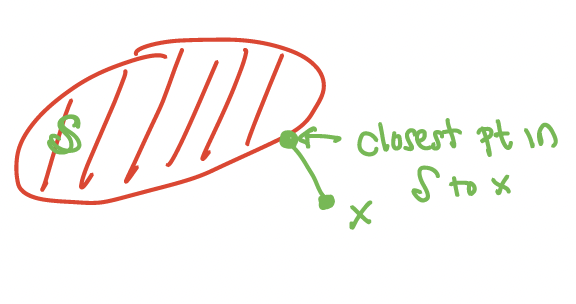
\includegraphics{projection}
  \caption{A projection}
\end{marginfigure}

  
\begin{definition}[Projection on a Set]
Let $S \in \mathbb{E}$ be non empty and $x \in \mathbb{E}$, then the projection of $x$ on $S$ is 
  $$P_S(x) := \argmin_{y \in S} \|x-y\| \subset S $$
\marginnote{We say that $P_S(x)$ is a subset of $S$ because it could contain more than one point (unless $S$ is convex). } 
\end{definition}
\begin{lemma} 
  Let $x \in \mathbb{E}$ and $S\subseteq \mathbb{E}$, then the following hold: 
  \begin{enumerate}
    \item[\it (i)] If $S$ is closed, then $P_S(x)\neq \varnothing;$ 
    \item[\it (ii)] If $S$ is convex, then $P_S(x)$ has at most one element. 
  \end{enumerate}
\end{lemma}
\begin{corollary}[Projection on closed, convex set]
  Let $C \subseteq \mathbb{E}$ be non empty, closed, and convex, then $P_C : \mathbb{E} \to C$ with $P_C(x) = x \iff x \in \mathbb{E} $. 
\end{corollary}
 \begin{theorem}[Projection Theorem] \label{label}
   Let $C \subseteq \mathbb{E}$ be non empty, closed, and convex, and let $x \in \mathbb{E}$. Then $\bar v = P_C(x)$ if and only if
   $$\bar v \in C \text{ and } \langle\bar v - x , v - \bar v \rangle \geq 0 \quad \forall v \in C $$
 \end{theorem}
 \subsection{Separation Theorem}
 \begin{theorem}[Separation Theorem] \label{SeparationThm}
   Let $C \subseteq \mathbb{E}$ be non empty, closed, and convex and let $x \notin C$. Then there exists an $s \in \mathbb{E} \setminus \{ 0 \}$ with
   $$\langle s , x\rangle > \sup_{v\in C}\langle s, v \rangle  $$ 
 \end{theorem}
 \begin{remark} 
   Under the assumptions of Theorem \ref{SeparationThm}, the following hold: 
   \begin{enumerate}
     \item[\it (a)] $s$ can be substituted for $-s$ and thus $\langle s , x\rangle <\inf_{v\in C}\langle s, v \rangle $;
     \item[\it (b)] By positive homogeneity, we can assume \textit{wlog} that $\| s\| =1$ ;
     \item[\it (c)] A reformulation of the statement of the separation theorem is that for $C \subseteq \mathbb{E}$ non empty, closed, and convex and $x \notin \mathbb{E}$, there exists an $s \in \mathbb{E}\setminus \{0\}$ and $\beta \in \mathbb{R}$ such that
     $$\langle s, x \rangle > \beta \geq \langle s, v \rangle, \quad v \in C $$

   \end{enumerate}
 \end{remark}
 \section{Chapter 3: Convex Functions}
 \subsection{Definitions}
 \begin{definition}[Convex Function]
   A function $f: \mathbb{E}\to \mathbb{R}$ is said to be convex if $\epi f$ is a convex set. \sidenote{ Equivalently, $f$ is convex if $\epi_{<}f$ is a convex set, as proven in A2. }
 \end{definition}
\begin{proposition}[Hessian of a Convex Function] \label{Prop:Hessian}
  A twice differentiable function $f: \mathbb{R}^n \rightarrow \mathbb{R}$ is convex, if and only if the Hessian $\nabla^2 f(x)$ is positive semi-definite for all $x \in \mathbb{R}^n$.
  \begin{proof} \cite{grasmair}
Assume first that $f$ is convex and let $x \in \mathbb{R}^n$. Define moreover the function $g: \mathbb{R}^n \rightarrow \mathbb{R}$ setting
$$
g(y):=f(y)-\nabla f(x)^T(y-x) .
$$
Since the mapping $y \mapsto-\nabla f(x)^T(y-x)$ is affine, it follows that $g$ is convex. Moreover
$$
\nabla g(y)=\nabla f(y)-\nabla f(x)
$$
and
$$
\nabla^2 g(y)=\nabla^2 f(y)
$$
for all $y \in \mathbb{R}^n$. In particular, $\nabla g(x)=0$. Thus Corollary 6 implies that $x$ is a global minimiser of $g$. Now the second order necessary condition for a minimiser implies that $\nabla^2 g(x)$ is positive semi-definite. Since $\nabla^2 g(x)=\nabla^2 f(x)$ and $x$ was arbitrary, this proves that the Hessian of $f$ is positive semi-definite for all $x \in \mathbb{R}^n$.

Now assume that the Hessian $\nabla^2 f(x)$ of $f$ is positive semi-definite for all $x \in \mathbb{R}^n$. Let moreover $x, y \in \mathbb{R}^n$. Then Taylor's theorem implies that
$$
f(y)=f(x)+\nabla f(x)^T(y-x)+\frac{1}{2}(y-x)^T \nabla^2 f(x+t(y-x))(y-x)
$$
for some $0 \leq t \leq 1$. Since $\nabla^2 f$ is everywhere positive semi-definite, the quadratic term in this equation is always non-negative. Thus we can estimate
$$
f(y) \geq f(x)+\nabla f(x)^T(y-x) .
$$
And so, $f$ is convex.
\end{proof}
\end{proposition} 


\begin{remark} $  $
 \begin{enumerate}
   \item[\it (i)] Convex functions have convex level sets.
   \item[\it (ii)] The domain of convex functions is convex.
 \end{enumerate} 
 \end{remark}
\begin{definition}[Proper Convex Functions]
  A convex function is proper if $\dom f \neq \varnothing$ and $f(x)> -\infty \; \forall x \in \mathbb{E}$.
  \begin{marginfigure}
  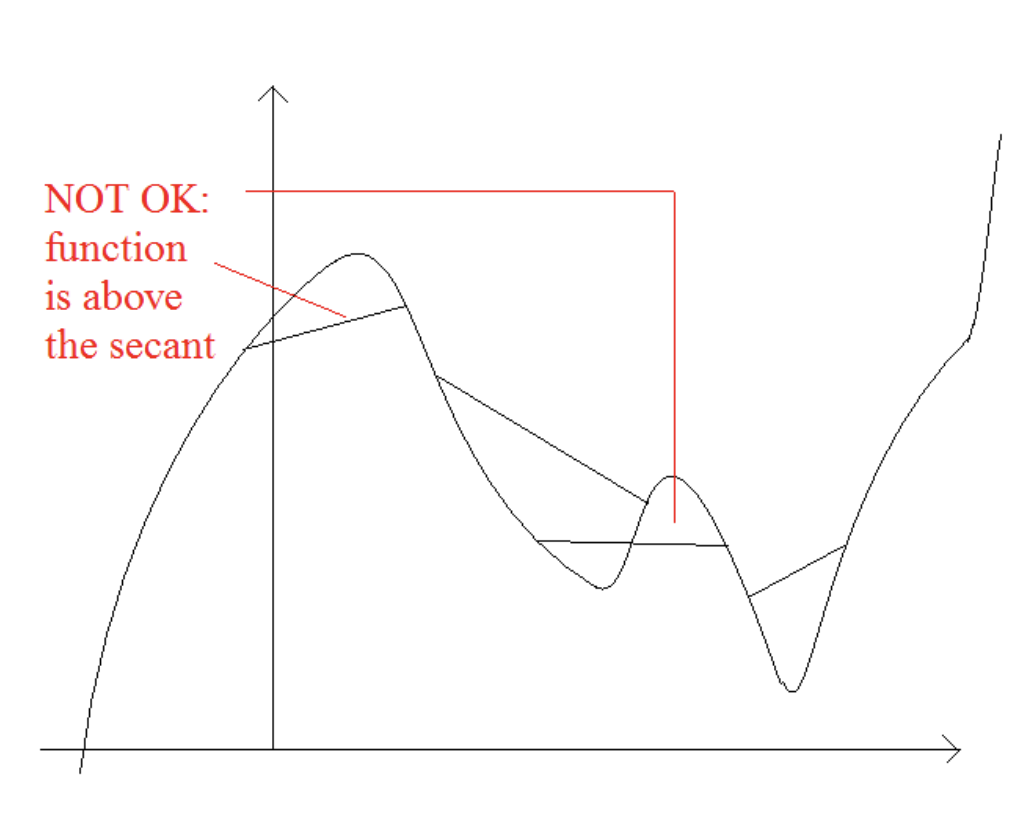
\includegraphics{nonConvex}
  \label{ConvexExamples2015}
  \caption{A nonconvex function does not lie below all of its secants.}
\end{marginfigure}

\end{definition}
 \begin{proposition}[Characterizing Convexity] \label{CharConvex}
   A function $f : \mathbb{E} \to \mathbb{R} \cup \{+\infty\}$ is convex if and only if $\forall x, y\in \mathbb{E} ,$ we have \cite{ConvexExamples2015} 
   \begin{equation} \label{charconv_eq}
    \begin{split}
    f(\lambda x + (1 - \lambda)y) \leq \lambda f(x)  + (1- \lambda) f(y) \quad \forall \lambda \in [0,1] 
    \end{split}
   \end{equation}

 \end{proposition}
 \begin{proposition}[Jensen's Inequality] \label{Jensens}
   A function $f: \mathbb{E} \to \mathbb{R} \cup \{ \infty \}$ is convex $\iff$  \marginnote{\textit{Jensen's Inequality} is a generalization of Proposition \ref{CharConvex}.}

   $$f \left( \sum^{p}_{i=1} \lambda_i x_i \right)\leq \sum^{p}_{i=1}\lambda_i f ( x_i), \quad x_i \in \mathbb{E},\; \lambda_i \in \Delta_p $$
  Where $\Delta_p :=\{ \lambda_i \in \mathbb{R}^p \mid \lambda \geq 0 , \; \sum \lambda_i = 1 \}$.
 \end{proposition}
 \begin{definition}[Convexity on a Set]
   Let $f: \mathbb{E}\to \mathbb{R} \cup \{\infty\}$, and $C \subset \dom(f)$ a convex, non-empty set. Then we call $f$ convex on $C$ if $\forall x, y \in C,$ (\ref{charconv_eq}) holds. 
\end{definition}
\begin{marginfigure}
  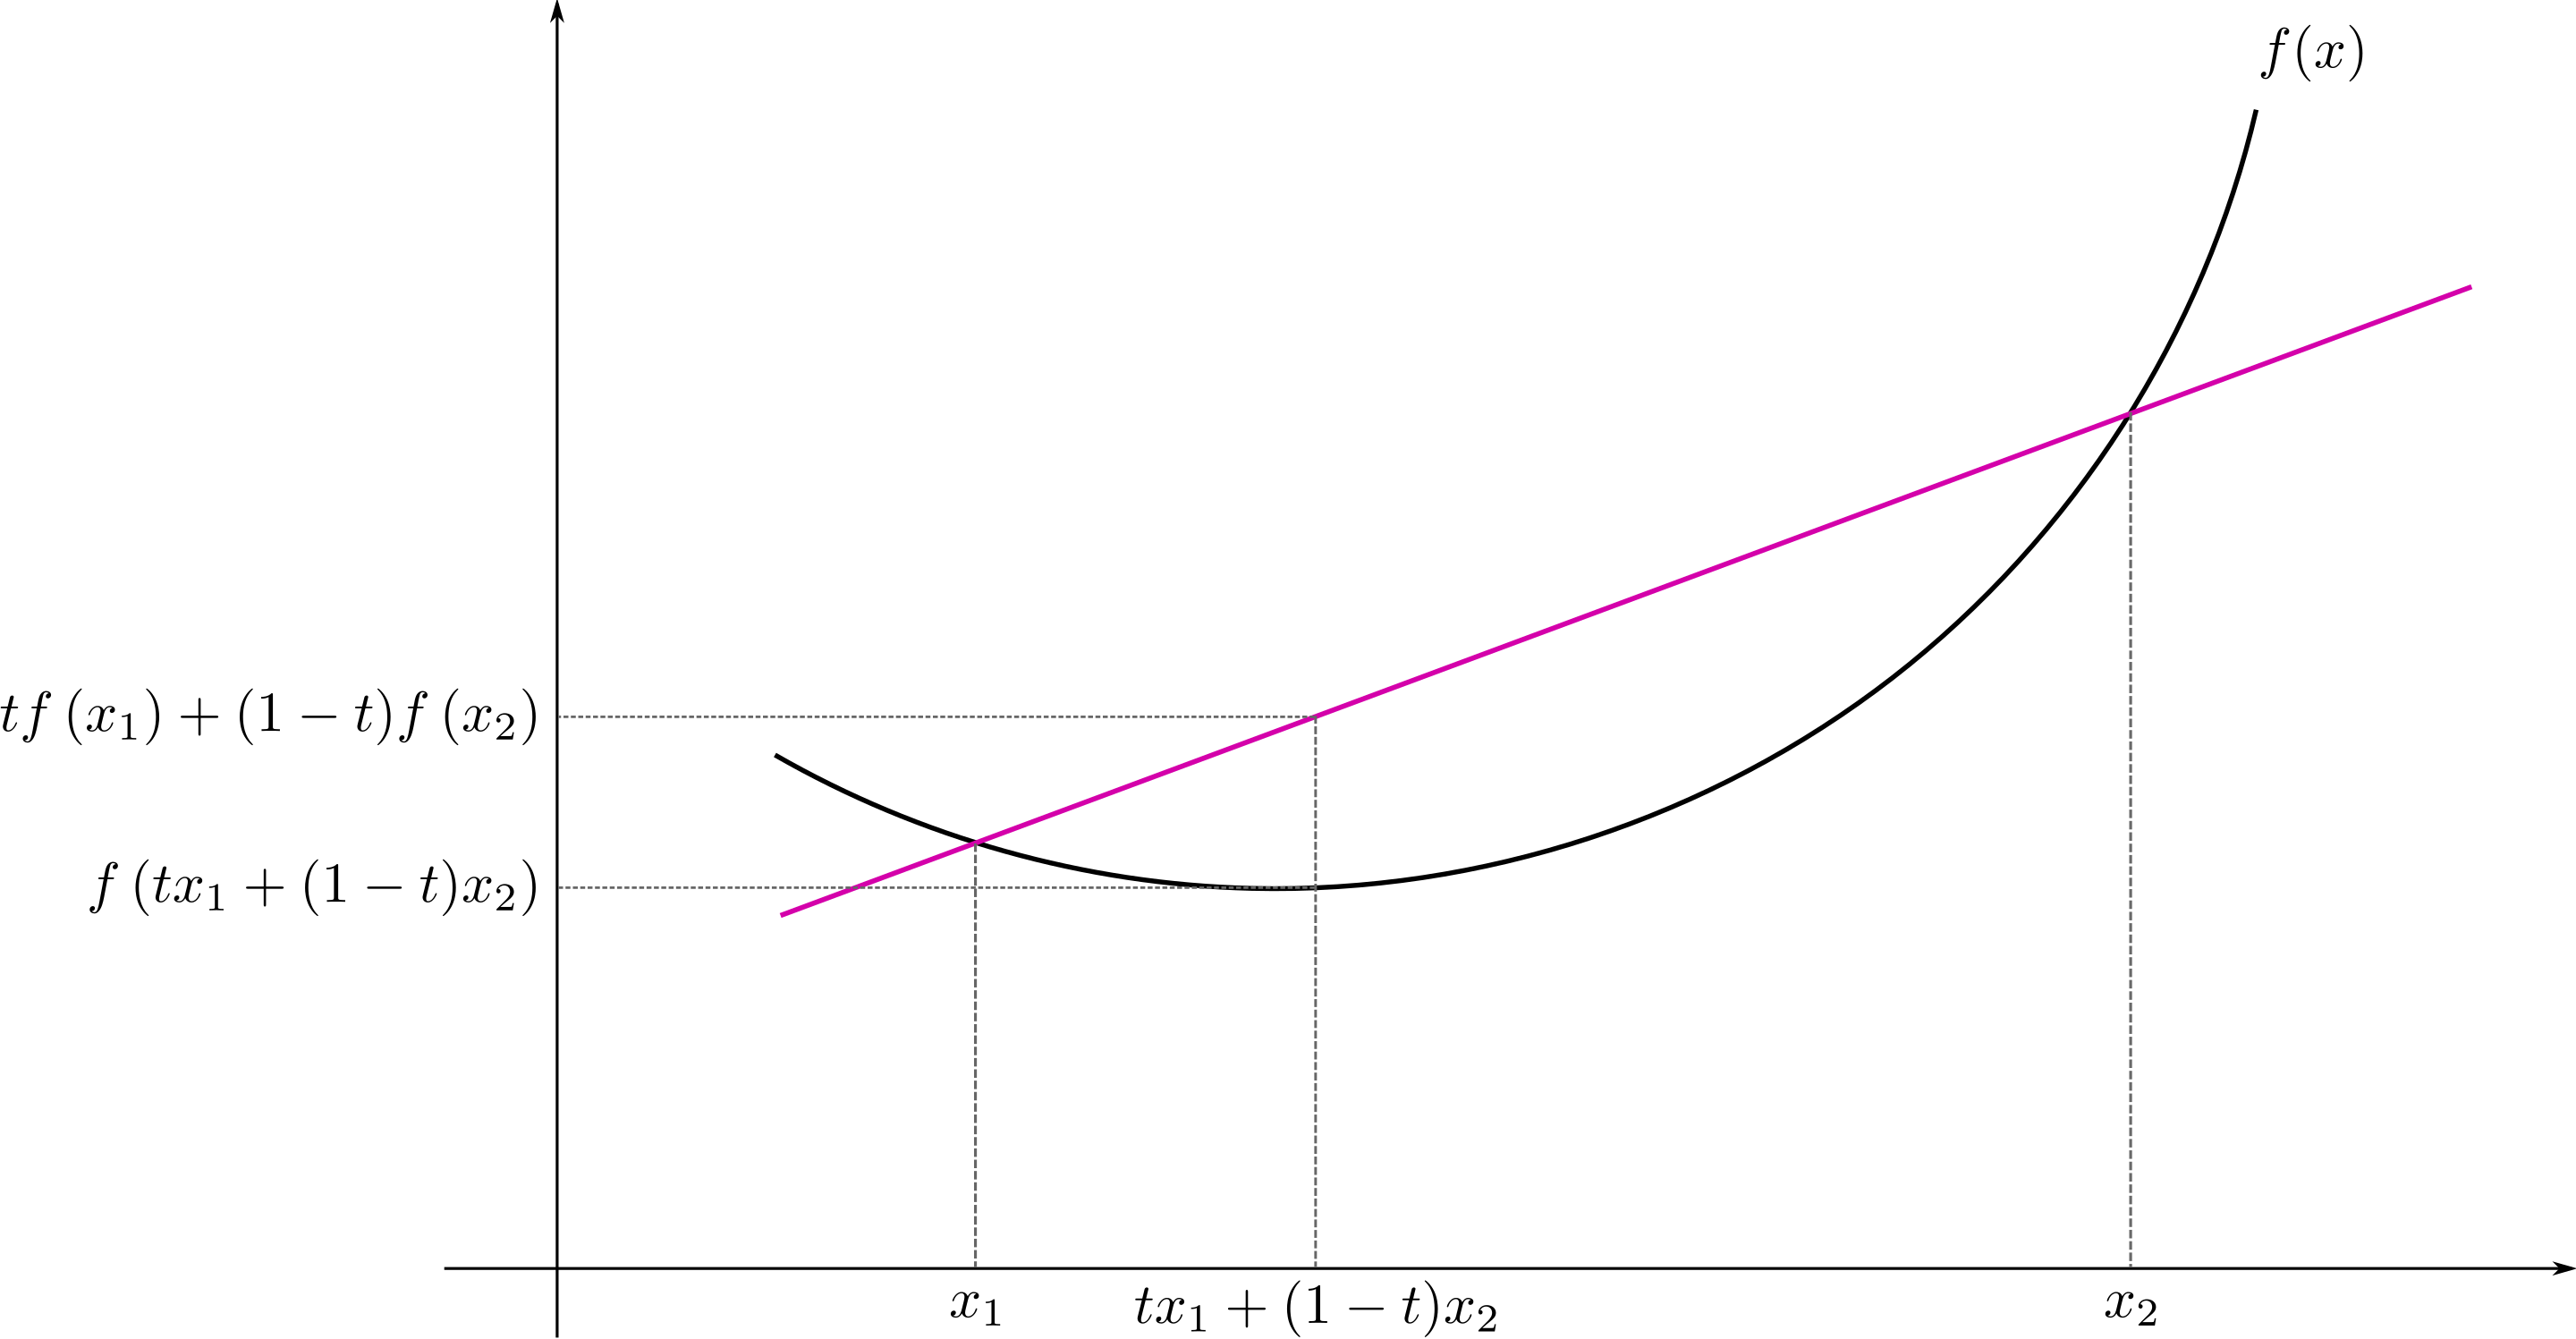
\includegraphics{convex}
  \caption{A convex function lies below all its secants.}
\end{marginfigure}
\begin{corollary} Let $f: \mathbb{E}\to \mathbb{R}\cup \{\infty\}$, then T.F.A.E. 
  \begin{enumerate}
    \item[\it (i)] $f$ is convex;
    \item[\it (ii)] $f$ is convex on its domain. 
  \end{enumerate} 
\end{corollary} 
\begin{remark}[Notation]
  Since we are mainly concerned with \textbf{proper, convex}, and sometimes \textbf{lower semicontinuous} functions, we shall use the following notation to denote such functions:
  $$\Gamma = \Gamma(\mathbb{E}) := \left\{ f: \mathbb{E} \to \mathbb{R} \cup \{\infty\} \mid f \text{ is proper \& convex } \right\} $$
  $$\Gamma_0 = \Gamma_0(\mathbb{E}) := \left\{ f: \mathbb{E} \to \mathbb{R} \cup \{\infty\} \mid f \text{ is proper, convex, \& lsc } \right\} $$

\end{remark}
\subsection{Stronger Notions of Convexity}
\begin{definition}[Strict Convexity]
  Let $f \in \Gamma$ and $C \subset \dom f$ a convex set, then $f$ is said to be \textbf{strictly convex} on $C$ if $$f(\lambda x + (1-\lambda)y)< \lambda f(x) + (1- \lambda )f(y),$$ 
  for any $\lambda \in (0,1),$ $x,y \in C $ s.t. $x \neq y$. For $C = \dom f$, we simply say that $f$ is strictly convex. 

\end{definition}
\begin{definition}[$\pmb{\sigma}$-Strong Convexity]
  Let $f \in \Gamma$ and $C \subset \dom f$ a convex set, then $f$ is said to be $\pmb{\sigma}-$\textbf{strongly convex} on $C$ if \marginnote{ The scalar $\sigma > 0$ is called the \textbf{modulus of strong convexity} of $f$ on $C$ }
  $$f(\lambda x + (1-\lambda)y)\leq \lambda f(x) + (1- \lambda )f(y)- \frac{\sigma}{2}\lambda (1-\lambda)\|x-y\|^2 ,$$ 
  for any $\lambda \in (0,1),$ $x,y \in C $ s.t. $x \neq y$. For $C = \dom f$, we simply say that $f$ is strongly convex. 
\end{definition}
\begin{remark} 
  Strongly convex $\implies$ Strictly convex, but the converse is not true. 
\end{remark}
\begin{proposition}[Characterizing Strong Convexity] \label{label}
  Let $f \in \Gamma$ and $C\subset \dom f$, then $f$ is strongly convex if and only if $f(x)- \frac{\sigma}{2} \| x \| ^2  $ is convex on $C$. 
  \begin{proof} 
    See assignment 2.
  \end{proof}
\end{proposition}
\subsection{Functional Operations Preserving Convexity}%
  \label{sub:Functional Operations Preserving Convexity}
  \begin{proposition}[Positive combinations of convex functions] \label{label}
    For $p\in \mathbb{N}$, let $f_i$ be convex (and lsc), $\alpha_i \geq 0$ for $i = 1,2,..., p$, then $$f = \sum^{p}_{i=1} \alpha_i f_i \quad \text{is convex (and lsc).} $$ 
    If in addition $\bigcap_{i = 1}^{p} \dom f_i \neq \varnothing$, then $f$ is also proper (i.e. $\dom f\neq \varnothing$). 
  \end{proposition}
  \begin{proposition}[Pointwise supremum of convex functions]
    For an arbitrary index set $\mathcal{I}$, let $f_i$ be convex (lsc) for all $i \in \mathcal{I}$. Then, the function $$f(x) = \sup_{i \in \mathcal{I}} f_i(x) \quad \forall x \in \mathbb{E} $$
    is convex (lsc).
  \end{proposition}
  \begin{definition}[Affine Functions]
    A function $F: \mathbb{E}_1 \to \mathbb{E}_2$ is called \textit{Affine} if 
    $$F(\alpha x + (1- \alpha ) y) = \alpha F(x) + (1- \alpha) F(y) \quad \forall x , y \in \mathbb{E}_1, \; \alpha \in \mathbb{R} $$
  \end{definition}
  \begin{remark} 
    $  $
    \begin{enumerate}
      \item Affine functions are convex and continuous.
      \item Linear functions are affine, and an affine function $F$ is linear if and only if $F(0) = 0$. 
      \item Affine images and preimages of convex sets are convex. 
    \end{enumerate}
  \end{remark}
  \begin{proposition}[Precomposition with an affine mapping]
    Let $H: \mathbb{E}_1 \to \mathbb{E}_2$ be affine and $g: \mathbb{E}_1 \to \mathbb{R}\cup \{\infty\}$ be convex (and lsc), then the function $f = g \circ H$ is convex (and lsc). 
    
  \end{proposition}
\section{Minimization and Convexity}
  \label{sec:Minimization and Convexity}
  \subsection{General Existence Result}%
    \label{sub:General Existence Result}
    \begin{definition}[Coercivity and Supercoercivity]
      Let $f: \mathbb{E} \to \overline {\mathbb{R}}$, then $f$ is called 
      \begin{enumerate}
        \item[\it (i)] \textbf{Coercive} if $$\lim_{\|x\| \to \infty} f(x) = + \infty $$
        \item[\it (ii)] \textbf{Supercoercive} if $$\lim_{\| x\| \to \infty} \frac{f(x)}{\|x\|} = + \infty $$ 
      \end{enumerate}
    \end{definition}
    \begin{proposition}  
      A function is coercive if and only if it is level bounded. 
      \begin{proof} 
        See assignment 2.
      \end{proof}
    \end{proposition}
    \begin{proposition}[Existence of Minimizers] \label{label}
      Let $f: \mathbb{E} \to \mathbb{R}\cup \{\infty\}$ be lsc and let $C\subset \mathbb{E}$ be closed such that $\dom f \cap C \neq \varnothing$. If one of the following holds,
      \begin{enumerate}
        \item[\it (i)] $f$ is \textit{coercive}; 
        \item[\it (ii)] $C$ is \textit{bounded}; 
      \end{enumerate}
      then $f$ has a minimizer over $C$. 
    \end{proposition}
    \begin{corollary}[Existence of Minimizers II]\marginnote{\color{red} Important corollary.}
      Let $f, g: \mathbb{R} \to \mathbb{R} \cup \{\infty\}$ be lsc such that $\dom f \cap \dom g \neq \varnothing$. If $f$ is coercive and $g$ is bounded from below, then $f+g$ is coercive and has a minimizer over $\mathbb{E}$.  
      
    \end{corollary}
    \subsection{Convex Optimization}%
      \label{sub:Convex Optimization}
      In the case of convex minimization, there is no difference between local and global solutions. 
      \begin{proposition} \label{label}
        Let $f\in \Gamma$, then every local minimizer over $\mathbb{E}$ is a global minimizer. 
      \end{proposition}
      \begin{corollary}[Minimizers in Convex Optimization]
        Let $f \in \Gamma$ and $C \subset \mathbb{E}$ be non-empty and convex. Then every local minimizer of $f$ over $C$ is a global minimizer of $f$ over $C.$
      \end{corollary}
      \begin{proposition} \label{label}
        Let $f \in \Gamma$, then $\argmin f$ is a convex set. 
      \end{proposition}
      \begin{corollary} Let $f \in \Gamma$ and $C \in \mathbb{E}$ convex. Then $\argmin_C f$ is convex. 
      \end{corollary}
      \begin{proposition}[Uniqueness of Minimizers]
        Let $f \in \Gamma$ be strictly convex, then $f$ has at most one minimizer. 
        \begin{proof} 
          Assignment 2.
        \end{proof}
      \end{proposition}
      \begin{proposition}[Minimizing the sum of Convex Functions]
        Le $f, g \in \Gamma_0$ such that $\dom f \cap \dom g \neq \varnothing.$ If one of the following holds, 
        \begin{enumerate}
          \item[\it (i)] $f$ is \textit{supercoercive};
          \item[\it (ii)] $f$ is coercive and $g$ is \textit{bounded from below}; 
        \end{enumerate}
        then $f+g$ is coercive and has a minimizer over $\mathbb{E}$. If $f$ or $g$ are strictly convex, then $f+g$ has a unique minimizer. 
      \end{proposition}
      \begin{theorem}[Parametric Minimization]
        Let $h: \mathbb{E}_1 \times \mathbb{E}_2 \to \mathbb{R}\cup \{\infty\} $ be convex. Then the \textbf{Optimal value function}
        $$\varphi:\mathbb{E}_1 \to \overline{\mathbb{R}}, \; \varphi(x) = \inf_{y \in \mathbb{E}_2} h(x,y) ,$$
        is convex. Moreover, the set-valued mapping 
        $$x \mapsto \argmin_{y \in \mathbb{E}_2} h(x,y) \subset \mathbb{E}_2, $$
        is convex-valued.
      \end{theorem}
\section{Infimal Convolution of Convex Functions}%
  \label{sec:Infimal Convolution of Convex Functions}
  \begin{definition}[Infimal Convolution]
    Let $f,g: \E \to \R \cup \{\infty\}$, then the function 
    $$f\# g : \E \to \overline{\R}, \quad (f\# g)(x) = \inf_{u \in \mathbb{E}} \{ f(u) + g(x -u) \} $$
    is called the \textbf{Infimal Convolution} of $f$ and $g$. \marginnote{We call the infimal convolution $f\#g$ \textbf{exact} at $x \in \E$ if $\argmin_{u\in \E} \{ f(u)+g(x-u) \}\neq \varnothing$. We simply say it is \textbf{exact} if it is exact everywhere. }
  \end{definition}
  \begin{lemma} 
    Let $f,g: \E \to \R \cup \{\infty\}$, then the following hold: 
    \begin{enumerate}
      \item[\it (i)] $\dom (f\#g) = \dom f + \dom g$;
      \item[\it (ii)] $f\#g  = g\#f$;
      \item[\it (iii)] $(f\#g)(x) \leq f(u) + g(x -u) \; \forall u \in \E.$
    \end{enumerate}
  \end{lemma}
  \begin{proposition}[Infimal convolution of convex functions]
    Let $f,g : \E \to \R \cup \{\infty\}$ be convex, then $f\#g$ is convex. 
    \begin{proof} 
      Assignment 3.
    \end{proof}
  \end{proposition}
  \begin{definition}[Distance function]
    Let $C\subset \E$, then the distance function $d_C = \delta_C \# \|\cdot \| $ is called the \textbf{Distance Function} to the set $C$. It holds that $$d_C(x) = \inf_{u \in C} \| x-u\|$$ 
  \end{definition}
  \begin{corollary}
    If $C\subset \E$ is closed and convex, we have 
    $$d_C (x) =  \| x - P_C(x)\| $$
    Moreover, the distance function of a closed set is convex by the above proposition.
    \begin{proof} 
      Follows from lemma 2.4.
    \end{proof}
  \end{corollary}
\begin{proposition}[Affine Minorization Principle]
  For $f \in \Gamma_0, $ there exists an \textit{Affine minorant}, namely, $\exists a\in \E , \; \beta \in \mathbb{R} \text{ s.t. }$ 
  $$ f(x) \geq \langle a, x \rangle + \beta \quad \forall x \in \E $$
\end{proposition}
\begin{theorem}[Infimal Convolution of $\Gamma_0$]
  Let $f , g \in \Gamma_0$ and suppose that one of the following holds: 
  \begin{enumerate}
    \item[\it (i)] $f$ is \textit{supercoercive;}
    \item[\it (ii)] $f$ is \textit{coercive and bounded from below;} 
  \end{enumerate}
  then $f \# g \in \Gamma_0$ and it is exact, i.e. $\forall x \in \E$, $\argmin_{u\in \E} \{ f(u)+g(x-u) \}\neq \varnothing$. 
  
\end{theorem}
\subsection{Moreau Envelopes and Proximal Mappings}%
  \label{sub:Moreau Envelopes and Proximal Mappings}
The Moreau envelope of a proper lower semi-continuous convex function $f \in \Gamma_0$, denoted $e_\lambda f$ is a smoothed version of $f$. It was proposed by Jean-Jacques Moreau in 1965. The Moreau envelope has important applications in mathematical optimization: minimizing over the Moreau enveloppe of $f$ and minimizing over $f$ are equivalent problems in the sense that the set of minimizers of $f$ and 
 $e_\lambda f$ are the same. However, first-order optimization algorithms can be directly applied to 
 $e_\lambda f$, since $f$ may be non-differentiable while $e_\lambda f$ is always continuously differentiable (given $f \in \Gamma_0$). Indeed, many proximal gradient methods can be interpreted as a gradient descent method over $e_\lambda f$.
  
  In this section, if a function $S$ maps points in a euclidian space $\E_1$ to subsets of another euclidian space $\E_2$, we denote it by $S: \E_1 \rightrightarrows \E_2$. 
  \begin{definition}[Moreau Envelope]
    Let $f: \E \to \overline{\R},$ the \textbf{Moreau envelope} of $f$ to the parameter $\lambda> 0$ is the function $e_\lambda f: \E \to \overline{R}$ defined by 
    $$e_\lambda f(x) = \inf_{u \in \mathbb{E}} \left\{f(u) + \frac{1}{2 \lambda} \| x - u\| ^2\right\} $$
  \end{definition}
  \begin{remark} 
  Notice that 
    $$e_\lambda f = f\# \left( \frac{1}{2\lambda } \| \cdot \|^2 \right) $$
  \end{remark}
  \begin{definition}[Proximal Mapping]
    Let $f: \E \to \overline{\R},$ the \textbf{Proximal mapping} to the parameter $\lambda >0$ of $f$ is the (possibly set-valued mapping) $P_\lambda f: \E \rightrightarrows \E$ defined by
    $$P_\lambda f(x) = \argmin_{u\in \E} \left\{f(u) + \frac{1}{2 \lambda} \| x - u\| ^2\right\}  $$
  \end{definition}
  \begin{proposition} 
    Let $f \in \Gamma_0$ and $\lambda >0$, then $e_ \lambda f \in \Gamma_0$ is finite-valued and $P_\lambda f$ is single valued. 
  \end{proposition}
  \begin{remark} 
    The Moreau envelope is a smoothing operation, namely, the Moreau envelope of a closed, proper, convex function is differentiable.
  \end{remark}
  \begin{proposition} \label{label}
      The \textit{proximal operator} of $f$ is related to the gradient of the \textit{Moreau envelope} of $f$ by the following identity 
      $$\nabla e_\lambda f = \frac{1}{\lambda} (x - P_\lambda f (x)) $$
  \end{proposition}
  \begin{example}[Moreau Envelope of an indicator function]
    Let $C \subset \E$ be nonempty, closed, and convex. Then 
    $$e_\lambda \delta _C (x) = \inf_{u \in C} \frac{1}{2 \lambda} \| x- u\| ^2 = \frac{1}{2\lambda } d_C^2 (x), $$
    i.e. $e_\lambda \delta_C$ is the \textit{distance function} and $P_\lambda \delta_C=P_C$ is the \textit{projection onto C.}  
  \end{example}
  \begin{remark} 
    For $f\in \Gamma_0$, $\lambda> 0$ and $x \in \E$, we have 
    $$e_\lambda f(x) = f(P_\lambda f(x)) + \frac{1}{2\lambda} \|x- P_\lambda f(x)\|^2 \leq f(u) + \frac{1}{2\lambda} \| x-u \|^2 \; \forall u \in \E, $$
    in particular, the Moreau envelope is a \textit{Minorant} for its input function.
  \end{remark}
  \begin{proposition} 
    Let $f \in \Gamma_0$ and let $x,p \in \E$. Then $p = P_1f(x) \iff \langle y -p , x-p \rangle + f(p) \leq f(y) \; \forall y \in \E.$ 
  \end{proposition}
  \begin{proposition}[Firm nonexpansiveness of prox-operator]
    Let $f \in \Gamma_0$, then $$\| P_1(x) - P_1 (y) \|^2 \leq \langle x-y , P_1f(x) - P_1 f(y) \rangle \; \forall x,y \in \E.$$ In particular, $\| P_1 (x) - P_1 (y) \| \leq \| x-y\| \; \forall x,y \in \E.$ That is, $P_1f$ is globally 1-Lipschitz continuous.
  \end{proposition}
  \begin{remark} 
    The above result extends to any $\lambda > 0$ through the identity 
    $$P_\lambda f = P_1 (\lambda f) $$
  \end{remark}
\section{Conjugacy of Convex Functions}%
  \label{sec:Conjugacy of Convex Functions}
  \subsection{Convex Hull of a Function}%
    \label{sub:Convex Hull of a Function}
    \textbf{Main Result:} Every proper, closed, convex function is the pointwise supremum of its affin minorants.
    \begin{theorem}[Envelope Representation of $\Gamma_0$]
       \begin{marginfigure}
  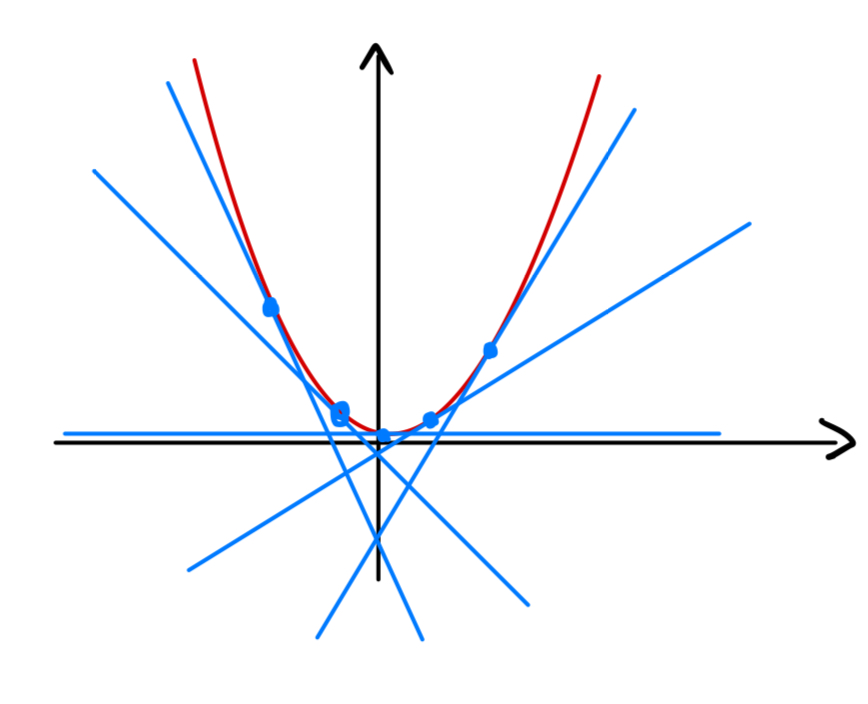
\includegraphics{AffineMinorant}
  \caption{Pointwise affine minorants.}
\end{marginfigure}

      Let $f \in \Gamma_0$, then $f$ is the pointwise supremum of all affine functions minorizing it, i.e. $$f(x) = \sup \{h(x) \mid h\leq f , \; h \text{ affine}\} $$ 
    \end{theorem}
    \begin{definition}[Convex Hull of a Function]
      Let $f: \E \to \overline{\R}$, then the pointwise supremum of all convex functions minorizing $f$, i.e. 
      $$(\conv f) (x) = \sup \{ h(x)\mid h \leq f, \; h \text{ convex} \}, $$
      is called the \textbf{convex hull} of $f$. Moreover, we define the \textbf{closed convex hull} of $f$ to be 
      $$(\overline{\conv} ) (x) = \sup \{h(x) \mid h \leq f , \; h \text{ lsc and convex}\} $$
    \end{definition}
    \begin{remark} 
      Since both convexity and lower semicontinuity are preserved under pointwise suprema, we find that $\conv f$ is the largest convex function that minorizes $f$ and $\overline{\conv} f$ is the largest lsc and convex function that minorizes $f$.  
    \end{remark}
    \begin{remark} 
      \begin{enumerate}
        \item[\it (i)] $\overline{\conv} f \leq \conv f \leq f$ and $ \overline{\conv} f  = \cl (\conv f) $; 
        \item[\it (ii)] We can also define the convex hull of $C \subseteq \E$ as 
        $$\conv C = \bigcap_{C \subset S,\; S\text{ convex}} S $$
        \item[\it (iii)] Every affine function $\E \to \R$ is convex and lsc, hence the functions $f , \; \cl f , \; \conv f, \overline{\conv} f$ have the same affine minorants. 
      \end{enumerate}
    \end{remark}
    \begin{corollary}[Affine envelope representation of $\overline{\conv}$] \label{affineEnvelope} Let\\  ${f: \E \to \overline {\R}}$ be proper and minorized by an affine function. Then $\overline{\conv} f$ is the pointwise supremum of all affine functions minorizing $f$, i.e. 
      $$(\overline{\conv} f) (x) = \sup\{h (x) \mid h \leq f, \; h \text{ affine}\} $$
      
    \end{corollary}
    \subsection{Fenchel Conjugate}%
      \label{sub:Fenchel Conjugate}
      \begin{definition}[Fenchel Conjugate]
        Let $f: \E \to \overline{\R},$ then the \textbf{Fenchel Conjugate} (or simply conjugate) of $f$ is the function \\ $f^* : \E \to\overline{R}$ defined by 
        $$f^* (y) = \sup _{x \in \E} \{ \langle x,y \rangle - f(x) \} $$
        The function $f^{**} = (f^*)^*$ is called the Fenchel biconjugate of $f$. 
      \end{definition}
      \begin{proposition}[Fenchel-Young Inequality]
        Let $f: \E \to \overline{R},$ then  
        $$f(x) + f^*(y) \geq \langle x,y \rangle \; \forall x,y \in \E $$
      \end{proposition}
      \begin{remark} 
        $f\leq g \implies f^* \geq g^* $ and in particular $f\geq f^{**}$.
      \end{remark}
      \noindent \textbf{Motivation for the Fenchel Conjugate.} Let $F: \E \to \overline{R}$, we notice that 
      $$\epi f^* = \{(y, \beta) \mid \langle x, y \rangle - f(x) \leq \beta \; \forall x \in \E\} $$
      This means the conjugate of $f$ is the function whose epigraph is the set
of all $(y, \beta )$ defining affine functions $x \mapsto \langle y, x \rangle - \beta$  that minorizes $f$. In view of Corollary \ref{affineEnvelope}, if $f$ is proper and has an affine minorant, the pointwise supremum of these affine mappings is the closed, convex
hull of $f$, i.e. through its epigraph, $f^*$ encodes info about $f$ and its
closed convex hull. Since $$f^* (y) = \sup \{ \langle x,y \rangle -f(x) \} = \sup_{(x, \alpha) \in \epi f} \{\langle y, x \rangle - \alpha \} \; \forall y\in \E,$$ we also have 
$$\epi f^* = \{(y, \beta) \mid \langle x,y \rangle - \alpha \leq \beta , \; (x, \alpha)\in \epi f\} $$
\begin{theorem}[Fenchel-Moreau Theorem] Let $f: \E \to \overline{R}$ be proper and have an affine minorant,then the following hold: 
  \begin{enumerate}
    \item[\it (i)] $f^*, \; f^{**}$ are closed, proper, and convex; 
    \item[\it (ii)] $f^{**} = \overline{\conv} f$;
    \item[\it (iii)] $f^* = (\conv f)^* = (\cl f)^* = (\overline{\conv}f)^*.$
  \end{enumerate}
\end{theorem}
\begin{remark} 
  $f\geq f^{**}$ for any function $f: \E \to \overline{\R}$ that has an affine minorant, and it holds that $f^{**} = f$ if and only if $f$ is closed and convex. 
\end{remark}

\begin{proposition}[Conjugacy of infimal convolution] Let $f, g: \mathbb{E} \rightarrow \overline{\mathbb{R}}$, then
$$
(f \# g)^{*}=f^{*}+g^{*} \text {. }
$$
  \begin{proof}(\text{\color{red}HWK})
  \begin{equation*}
    \begin{split}
      (f \# g)^*(x) &= \sup_{v \in \mathbb{E}}\{\langle v, x \rangle - (f \# g) (v)\}\\
      &= \sup_{v \in \mathbb{E}}\{\langle v, x \rangle -  \inf_{u \in \mathbb{E}} \{ f(u) + g(v-u) \}\} \\ 
      &= \sup_{v \in \mathbb{E}}\{\langle v, x \rangle   + \sup_{u \in \mathbb{E}} \{ -f(u) - g(v-u) \}\}  \\ 
      &= \sup_{v,u \in \mathbb{E}}\{\langle v, x \rangle   + -f(u) - g(v-u) \} \\ 
      &= \sup_{v,u \in \mathbb{E}}\{\langle v-u, x \rangle +  \langle u, x \rangle -f(u) - g(v-u) \} \\
      &= \sup_{v,u \in \mathbb{E}}\{(\langle v-u, x \rangle -g(v-u) )+  (\langle u, x \rangle-f(u)) \} \\ 
      &= \sup_{v \in \mathbb{E}}\{ \langle v,x\rangle -f(v) \} + \sup_{v \in \mathbb{E}}\{ \langle v,x\rangle -g(v) \}\\ 
      &= f^*(x) + g^*(x)
    \end{split}
  \end{equation*}
\end{proof}  
\end{proposition}
\begin{corollary}[Conjugacy correspondence]
  The Fenchel transform induces a 1-1 correspondence on $\Gamma_0$. For $f, g \in \Gamma_0$, $f$ is the conjugate to $g$ if and only if $f$ is the conjugate to $f$.  
\end{corollary}
\begin{proposition}[Elementary cases of Conjugacy]
  Let $f: \E \to \overline{\R} ,$ then the following hold: 
  \begin{enumerate}
    \item $(f-\langle{a}, \cdot\rangle)^{*}=f^{*}((\cdot)+{a})$ for ${a} \in \mathbb{E}$;
\item $(f+\gamma)^{*}=f^{*}-\gamma$ for all $\gamma \in \mathbb{R}$;
\item $(\lambda f)^{*}=\lambda f^{*}\left(\frac{(\cdot)}{\lambda}\right)$ for all $\lambda>0$;
\item Let $g, h: \E \to \overline{\R}$ be proper, closed, convex functions, and let $A \E \to Y$ be a linear map. Define $F(x,y) = h(Ax + y) + g(x).$ Then, $$F^* (x,y ) = g^*(x- A^*y) + h^*(y), $$ 
    where $A^*$ is the adjoint map. 
  \end{enumerate}
  \begin{proof} $  $
    \begin{enumerate}
    \item   
    \begin{equation*}
      \begin{split}
        f^*(\cdot + a) &= \sup_{x \in \mathbb{E}} \left\{ \langle x, \cdot + a \rangle - f(x) \right\} \\ 
        &= \sup_{x \in \mathbb{E}} \left\{ \langle x, \cdot \rangle + \langle x, a \rangle - f(x) \right\}\\ 
        &= \sup_{x \in \mathbb{E}} \left\{ \langle x, \cdot \rangle - (f- \langle a, \cdot \rangle )(x)\right\}\\ 
        &= (f-\langle a, \cdot \rangle)^*
      \end{split}
    \end{equation*}
  
  \item   
    \begin{equation*}
      \begin{split}
        (f+ \gamma)^* &= \sup_{x \in \mathbb{E}} \left\{ \langle x, \cdot \rangle - (f+ \gamma)(x) \right\}\\ 
        &= \sup_{x \in \mathbb{E}} \left\{ \langle x, \cdot \rangle - f(x) - \gamma \right\}\\
        &= \sup_{x \in \mathbb{E}} \left\{ \langle x, \cdot \rangle - f(x)\right\} - \gamma\\
        &= f^* - \gamma
     \end{split}
    \end{equation*}
  \item  \begin{equation*}
    \begin{split}
      (\lambda f)^* &= \sup_{x \in \mathbb{E}} \left\{ \langle x, \cdot \rangle - (\lambda f)(x)\right\} \\ 
      &= \sup_{x \in \mathbb{E}} \left\{ \lambda \left(\frac{\langle x, \cdot \rangle}{\lambda} - f(x)\right)\right\} \\ 
      &=  \lambda \sup_{x \in \mathbb{E}} \left\{ \frac{1}{\lambda}\langle x, \cdot \rangle - f(x)\right\} \\ 
      &= \lambda \sup_{x \in \mathbb{E}} \left\{ \langle x, \frac{(\cdot) }{\lambda} \rangle - f(x)\right\} \\ 
      &= \lambda f^{*}\left(\frac{(\cdot)}{\lambda}\right)
    \end{split}
  \end{equation*}
    
\end{enumerate}
\end{proof}

\end{proposition}

\section{Differential Theory}%
  \label{sec:Differential Theory}
  We will study differentiability of convex functions and, in
particular, develop tools where differentiability is lacking. 
{\subsection{Convex Subdifferential}%
  \label{sub:Convex Subdifferential}
  Some operations on convex functions destroy differentiability but preserve convexity - such as the max operation. In these situations, subgradients offer a method of generalizing gradients for optimizing convex functions that are not necessarily differentiable (where gradient descent does not work).
For motivational purposes, we consider the following result on smooth, convex functions. 
\begin{proposition} Let $C \subset \E$ be open and convex and let $f: \E \to \R$ be continuous and differentiable on $C.$ Then $f$ is convex on $C$ if and only if $$f(x) \geq f(\bar x) + \langle \nabla f(\bar x ), x- \bar x \rangle \; \forall x, \bar x \in C $$ 
 \begin{proof} 
  Assignment 3.
 \end{proof} 
\end{proposition}
\begin{definition}[Convex Subdifferential]
  Let $f: \E \to \overline{\R}$ and $\bar x \in \E$, then $g \in \E$ is called a \textbf{subgradient} of $f$ at $\bar x$ if $$f(x) \geq f(\bar x)  +\langle g, x- \bar x \rangle \; \forall x \in \E .$$ \marginnote{The subdifferential $\partial f(\bar x)$ of $f: \E \to \overline{\R}$ at $\bar x \in \E$ contains exactly the slopes of all affine minorants of $f$ that coincide with $f$ at $\bar x.$ }
  The set $$\partial f(\bar x) = \{v \in \E \mid f(x) \geq f(\bar x) + \langle v, x- \bar x \rangle \; \forall x \in \E \}$$
  of all subgradients is called the convex \textbf{Subdifferential} of $f$ at $\bar x$. 
\end{definition}

\begin{remark} 
  Note that we did not restrict ourselves to convex functions
in the above definition but the class $\Gamma$ is where the subdifferential is most meaningful.
\end{remark}
\begin{remark} 
  If a function is differentiable at $\bar x$, then the \textit{subdifferenial} $\partial f(\bar x)$ contains only one subgradient ($\nabla f$).

\end{remark}
\begin{example}[Subdifferential of Indicator Function]
  Let $C \subset \E$ be convex and $\bar x \in C$, then 
  \begin{equation*}
    \begin{split}
      g \in\partial \delta_C (\bar x) &\iff \delta_C (x) \geq \delta_C (\bar x) + \langle g , x- \bar x \rangle \; \forall x \in \E \\ 
      &\iff 0 \geq \langle g , x- \bar x \rangle \; \forall x \in C 
    \end{split}
  \end{equation*}
  that is, $$\partial \delta_C (\bar x) = \{ v \in \E \mid \langle v , x- \bar x \rangle\leq 0   \; \forall x \in C \}$$
  The latter set is called the \textbf{Normal cone} of $C$ at $\bar x.$ 
\end{example}
  \begin{definition}[Normal Cone]
    If $C \subseteq \mathbb{E} $ is a set, then the \textbf{Normal cone} of $C$ at $\bar x$ is given by $$N_C(\bar y) = \{v \in \E \mid \langle y - \bar y, v \rangle \leq 0\; \forall y \in C\}$$
   \begin{marginfigure}
  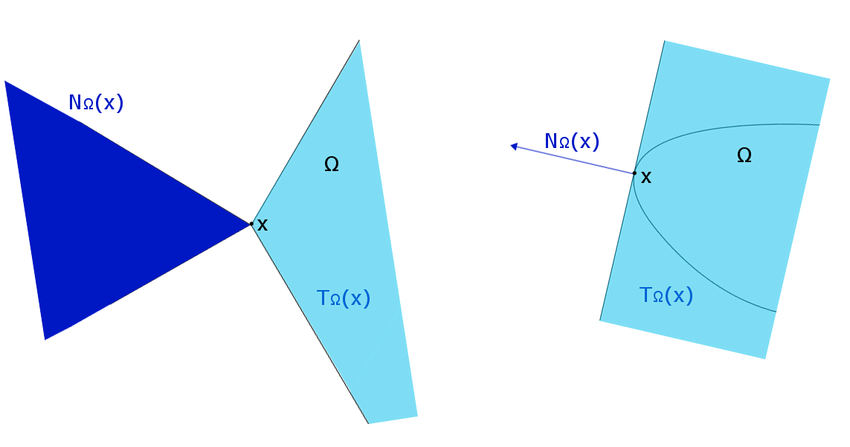
\includegraphics{Normal_cone}
  \caption{Normal cones.}
\end{marginfigure}

  \end{definition}
  \begin{proposition}[Properties of Subdifferentials] \label{label}
    Let $f: \mathbb{E}\to \mathbb{\bar R}$, then the following hold, 
    \begin{enumerate}
      \item[\it (i)] $\partial f(\bar x)$ is closed and convex for $\bar x \in \dom f$ 
      \item[\it (ii)] If $f$ is proper, then $\partial f (\bar x) = \varnothing\; \forall \bar x \notin \dom f$ 
      \item[\it (iii)] $0 \in \partial f(\bar x) \iff \bar x \in \argmin f$ 
      \item[\it (iv)] If $f$ is convex, then \marginnote{Recall that $N_{\epi f}$ denotes the normal cone of the epigraph of $f$. We note that if a function $f$ is differentiable at $x$, then the normal cone at $x$ contains only one vector. } $$\partial f (\bar x) = \{v \in \mathbb{E} \mid (v, -1) \in N_{\epi f}(\bar x , f(\bar x))\}$$ 

    \end{enumerate}
    \begin{proof} $  $
      \begin{enumerate}
        \item[\it (i)] We have 
        $$(\partial f)(\bar x) \bigcap^{}_{x \in \mathbb{E}} \{v \in \mathbb{E} \mid f(x) \geq f(\bar x) + \langle v , x - \bar x \rangle \} , $$
        since the intersection of convex, closed sets is also convex and closed.
        \item[\it (ii)] By proper, there exists an $x$ s.t. $f(x) < \infty$ and since $\bar x \notin \dom (f)$, we must have $f(\bar x) = \infty$. Using the definition of subgradient, we see that no $g$ satisfies the equation $f(x) \geq \langle g, x -\bar x\rangle + f(\bar x) $, thus $\partial f(\bar x ) = \varnothing$.
        \item[\it (iii)] By definition, we have $0 \in \partial f(x) \iff f(x) \geq f(\bar x) \; \forall x \in \mathbb{E}.$ Indeed, 

        $(\implies) \; 0 \in \partial f(\bar x) \implies f(x) \geq f(\bar x)$ by $f(x) \geq \langle g, x -\bar x\rangle + f(\bar x) $, for all $x$.

$(\impliedby) \; f(x) \geq f(\bar x) \; \forall x\implies f(x) \geq \langle 0 , x - \bar x \rangle + f(\bar x) \; \forall x \implies $ by definition of $f(x) \geq \langle g, x -\bar x\rangle + f(\bar x) $, $0 \in (\partial f)(\bar x)$. 
        \item[\it (iv)]
        \begin{equation*}
          \begin{split}
            v \in (\partial f) (\bar x) &\iff f(x) \geq f(\bar ) + \langle v, x - \bar x\rangle \; \forall x \in \dom f \\ 
            & \iff \alpha \geq f( \bar x ) + \langle v, x -\bar x\rangle \; \forall (x, \alpha) \in \epi f \\ 
            & \iff 0 \geq (f(\bar x)- \alpha ) + \langle v, x- \bar x\rangle  = \left\langle \begin{pmatrix}
              v \\ -1
            \end{pmatrix}, \begin{pmatrix}
              x- \bar x \\ \alpha - f(\bar x)
            \end{pmatrix}\right\rangle\; \forall (x , \alpha ) \in \epi f \\ 
            &\iff (v, -1) \in N_{\epi f } (\bar x , f(\bar x))
          \end{split}
        \end{equation*}
      \end{enumerate}
    \end{proof}
    
  \end{proposition}
 \begin{theorem}[Subdifferential and Conjugate Functions] \label{label}
  Let $f: \mathbb{E} \to \mathbb{\bar R}$, then T.F.A.E. 
   \begin{enumerate}
     \item[\it (i)] $y \in \partial f(x)$
     \item[\it (ii)] $x \in \argmax_z \{\langle z, y \rangle - f(z)\}$
     \item[\it (iii)] $f(x) + f^* (y) = \langle x, y \rangle$ (equality in \textit{Fenchel Young} if and only if $y\in \partial f(x)$) 
   \end{enumerate}
   If $f\in \Gamma_0,$ these are equivalent to 
   \begin{enumerate}
     \item[\it (iv)] $x \in (\partial f^*) (y)$ 
     \item[\it (v)] $y \in \argmax_w \{ \langle x, w \rangle - f^* (w)\}$
   \end{enumerate}
   \begin{proof} 
     \begin{equation*}
      \begin{split}
        y \in (\partial f)(x) &\iff f(z) \geq (x) + \langle y, z-x\rangle \quad \forall z \\ 
        & \iff \langle y, x \rangle - f(x) \geq \langle y, z\rangle - f(z) \quad \forall z \\ 
        & \iff \langle y, x \rangle - f(x) \geq  \sup_z \{  \langle y, z\rangle - f(z)  \} \\ 
        &\iff \langle y, x \rangle - f(x) \geq f^*(y)
      \end{split}
     \end{equation*}
     And, because \textit{Fenchel Young} gives the reverse inequality, it must be true that we had equalities instead of inequalities the whole time. For \textit{(iv)} and \textit{(v)},  apply the same reasoning to $f^*$ and use that $f^{**} = f$ if $f\in \Gamma_0.$  
   \end{proof}
 \end{theorem} 
  \begin{remark} 
    $(i)$ and $(iv)$ $\iff (\partial f^*) = (\partial f)^{-1}$. 
  \end{remark}
\subsection{Directional Derivative of Convex Functions}%
  \label{sub:Directional Derivative of Convex Functions}
 \begin{definition}[Directional Derivative]
   let $f: \mathbb{E} \to \mathbb{\bar R}$ be proper. For $x \in \dom f $, we say that $f$ is directionally differentiable at $x$ in the direction $d \in \mathbb{E}$ if $$\lim_{t \downarrow 0} \frac{f(x+ td)- f(x)}{t} \text{ exists } $$ 
   In this case, we call $$f^\prime (x; d) = \lim_{t \downarrow 0} \frac{f(x+ td)- f(x)}{t} $$
   the directional derivative of $f$ at $x$ in direction $d.$ 
 \end{definition} 
 \begin{remark} 
   If $f$ is differentiable at $x \in \operatorname{int} (\dom f),$ then $$f^\prime (x;d) = \langle \nabla f(x) , d\rangle \quad \forall d $$ 
 \end{remark}
 \begin{example}[]
   Let $f : \E \to \R$, $f(x) = \| x\|$, then 
   \begin{equation*}
    \begin{split}
      f^\prime ( x; d ) =  
      \begin{cases}
        \left\langle \frac{x}{\|x\|},d \right\rangle, &\text{ if } x \neq 0\\
        \| d\| , &\text{ otherwise.}
      \end{cases}
    \end{split}
   \end{equation*}
   for $x \neq 0, \;f$ is differentiable, so compute $\nabla f$. For $x = 0, $
   $$\lim_{t \to 0} \frac{\|0 + td \| - \| 0\|}{t}  = \lim_{t \to 0} \| d\| = \| d\| $$
   \end{example}
 Next, we show that 
   \begin{enumerate}
     \item[\it (i)] $f^\prime (x; d)$ exists; 
     \item[\it (ii)] positively homogeneous, finite, and convex in the interior of the domain. 
   \end{enumerate}
   if $f \in \Gamma$. Let $h : \E \to \R \cup \{\infty\}$, we call $h$ positively homogeneous if $$h(\lambda x ) = \lambda h(x) \quad \forall x \in \E , \; \lambda \geq 0 $$
   \textbf{HWK:} show $h$ is convex and homogeneous if and only if 
   $$h( \lambda x +\mu y  ) \leq \lambda h(x) + \mu h(y)\quad \forall x,y \in \E, \; \mu, \lambda \geq 0 $$
   This property is called \textbf{sublinearity}. 
\begin{remark} 
  Observe that if $h$ is positive homogeneous, then $h(0) = 0$, and $h$ satisfies 
  $$-h(x )= h(-x) \quad \forall x \in \E $$
  since $h(0) =0 = h(-x+x) \overset{sublinearity}{\leq} h(x) + h(-x)$
\end{remark}
\begin{proposition}[Directional Derivative of Convex Functions] \label{prop:dirdercon}
  Let $f \in \Gamma$, $ x\in \dom f$ and $ d\in \E$ direction. Define $$t\in \R \setminus \{0\} \quad q(t) = \frac{f(x+ td) - f(x)}{t}  $$ 
  then, the following hold, 
  \begin{enumerate}
    \item[\it (i)] $q(-t) \leq q(-s ) \leq q(s) \leq q(t)$ ;
    \item[\it (ii)] We have $f^\prime (x; d) = \inf_{t> 0} q(t).$ In particular, $f^\prime(x;d)$ exists at least in the extended sense. 
    \item[\it (iii)] $\dom (f^\prime (x; \cdot {})) = \R_+ (\dom f - x) := \{\lambda y \mid \lambda \in \R_+ , \; y \in \dom (f -x)\}$
    \item[\it (iv)] If $x \in \inte (\dom f)$, the function $f^\prime (x ; \cdot )$ is finite valued, positively homogeneous, and convex (also sublinear).
  \end{enumerate}
  \begin{proof} 
    $  $
    \begin{enumerate}
      \item[\it (i)] HWK. (use convexity, choose the right $\lambda$)
      \item[\it (ii)] Since the infimum always exists, $\inf_{t\downarrow 0} q(t)$ exits. By (i), $q(t)$ decreases as $t \downarrow 0$, so $$\inf_{t> 0} q(t) = \lim_{t\downarrow 0} q(t) = f^\prime (x; d)$$
      \item[\it (iii)] $d \in \dom f^\prime (x; \cdot )$, 
      \begin{equation*}
        \begin{split}
          &\iff \exists t >0 \quad \frac{f(x + td ) - f(x)}{t} < \infty \\ 
          &\iff \exists t>0 \quad f(x + td ) - f(x) \leq \infty \\ 
          &\iff \exists t > 0 \quad x + td \in \dom f \\ 
          & \iff d\in \R_+ (\dom f - x)
        \end{split}
      \end{equation*}
      \item[\it (iv)] Take $0 < s< t$ and observe 
      $$q(-t) \leq q(-s) \leq q(s) \leq q(t) $$
      If $x \in \inte (\dom f)$, we can choose $t$ sufficiently small so that $x \pm td \in \inte (\dom f)$. Thus, $q(t)$ and $q(-t)$ are finite. Hence, $$-\infty < q(-t) \leq q(-s) \leq f^\prime (x; d) = \lim_{s\downarrow 0} q(s ) \leq q(t)< \infty $$
      And, since $d$ was arbitrary, $f^\prime (x; d)$ is finite valued. Check that $f^\prime (x;d)$ is positively homogeneous. For convexity, let $t> 0$, $d,h\in \E$ and $\lambda \in [0,1]$. By convexity of $f,$
      \begin{equation*}
        \begin{split}
          \frac{f(x + t(\lambda d + (1- \lambda ) h)) -f(x)}{t} &=  \frac{f(\lambda(x + td) +  (1- \lambda ) (x + th)) -f(x)}{t}\\ 
          &\leq \frac{\lambda f(x + td) + (1- \lambda)f(x+ th) - (\lambda + (1- \lamdba))f(x)}{t} \\ 
          &= \frac{\lambda(f(x+ td) - f(x)) + (1-\lambda )(f(x+ th) -f(x))}{t} 
        \end{split}
      \end{equation*}
      Now, take $t \downarrow 0 $ to get directional derivatives.  
    \end{enumerate}
  \end{proof}
\end{proposition}
\begin{definition}
  For sublinear functions $h : \E \to \R \cup \{\infty \}$, we define the linearity space, 
  $$\lin h = \{x \in \E \mid h(-x) = - h(x)\} $$
\end{definition}
\begin{lemma} \label{lemsublin}
  Let $h: \E \to \R \cup \{\infty\}$ be sublinear, then the following hold, 
  \begin{enumerate}
    \item[\it (i)] The linearity space $\lin h$ of $h$ is the subspace on which $h$ is linear. 
    \item[\it (ii)] For $\bar x \in \inte (\dom h )$ and $q = h^\prime (\bar x ; \cdot ) $, we have 
    \begin{enumerate}
      \item $q(\lambda \bar x) = \lambda h(\bar x) \; \forall \lambda \in \R$
      \item $q\leq h $ 
      \item $\lin q > \lin h + \text{span}\{\bar x\}$
    \end{enumerate}

  \end{enumerate}
  \begin{proof} 
    HWK.
  \end{proof}
\end{lemma}
\begin{theorem}
  Let $f \in \Gamma$, then the following hold, 
  \begin{enumerate}
    \item[\it (i)] For all $\bar x \in \E$, $$\partial f(\bar x) = \{ s \mid \langle s, d \rangle \leq f^\prime (\bar x ; d) \} \; \forall d$$
    \item[\it (ii)] For all $\bar x \in \operatorname{int} (\dom f),$ we have $$f^\prime (\bar x; d) = \max_{s\in \partial f(\bar x) } \langle s, d \rangle $$
    In particular, $(\partial f)(\bar x) $ is non empty. 
  \end{enumerate}
  \begin{proof} 
    (i) is in HWK. \newline 
    (ii) Let $d \in \E = \R^n ,$ by part (i), we need to show that $\exists s \in \partial f(\bar x )$ such that $\langle s, d \rangle = f^\prime (\bar x ; d)$. Now let $\{b_1,...,b_n\}$ be a basis of $\E$ with $b_1 = d$ if $d \neq 0$. If $d= 0$, then any basis of $\R^n$. We define $p_0, p_1, ..., p_n$ by
    $$p_0= f^\prime(\bar x; \cdot ),\quad p_k = p^\prime _{k -1}(b_k ; \cdot) \; \forall k= 1,...,n $$ 
    By proposition \ref{prop:dirdercon}, $p_k$ is finite and sublinear. 

    $$\lin p_k > \lin p_{k-1} + \text{span}\{b_k\}\quad k = 1,...,n $$
    Thus, 
    $$\lin p_n = \E, $$
    i.e. by lemma \ref{lemsublin} part (a), $p_n$ is linear on $\E$. Therefore, there exists an $s$ such that $p_n(\cdot {}) = \langle s, \cdot \rangle$ (Riesz representation Theorem). Part (ii) of lemma \ref{lemsublin}, (b) implies 
         $$ \langle s, \cdot \rangle = p_n \leq p_{n-1} \leq ... \leq p_0 = f^\prime (\bar x ; \cdot ),$$
          Hence, 
    $$\langle s, x -\bar x \rangle = p_n (x -\bar x) \leq p_0 (x -\bar x ) = f^\prime (\bar x , x - \bar x) \overset{\ref{prop:dirdercon}}{\leq} f(\bar x + (x - \bar x)) - f(\bar x ) = f(x) -f(\bar x) $$
    for any $x$, thus $s \in \partial f(\bar x)$. If $d = 0$, then $ f^\prime (\bar x; 0) = \langle s, 0 \rangle. $ If $d \neq 0,$ i.e. $b_1 = d$, then by lemma \ref{lemsublin} (ii)(a), and definition of $p_1,$ we get 
    \begin{equation*}
      \begin{split}
        p_n(d)\leq p_0 (d) = p_0(b_1) &= - p_1(-b_1) = -p_1(-d)\\ 
&\leq -p_n (-d) = p_n (d) \\ 
        \implies & p_n(d)= p_0 (d)\\ 
        \implies & \langle s, d\rangle = f^\prime (\bar x ; d )
      \end{split}
    \end{equation*}
    
  \end{proof}
\end{theorem}
\subsection{Continuity Properties}%
  \label{sub:Continuity Properties}
  \textbf{Main result:} The \textit{Subdifferential} operator $\partial f : \E\rightrightarrows \E$ of a closed, proper and convex function has a closed graph 
  $$\operatorname{gph} \partial f := \{ (x,y) \in \E \times \E \mid y \in \partial f(x) \},$$
  which is referred to as the \textbf{outer semi-continuity } of $f.$
  \begin{corollary} Let $f \in \Gamma_0$  and suppose $\{ x_n \}\to x $, and $\{y_n \in \partial f(x_n)\}\to y$. Then, $y \in \partial f(x)$, i.e. $\operatorname{gph}\partial f \in \E \times \E $ is closed. 
  \end{corollary}
  \begin{theorem}\label{thm:lipcont}
    A function $f \in \Gamma$ is locally \textbf{Lipschitz} at every $x \in \operatorname{int}(\dom f).$ 
  \end{theorem}
  \begin{proposition} 
    Let $F: \mathbb{E}_{1} \rightarrow \mathbb{E}_{2}$ be locally \textbf{Lipschitz} at every point of the compact set $C$, i.e., for every $\overline{\boldsymbol{x}} \in C$ there exists $L=L(\overline{\boldsymbol{x}})$, $\varepsilon=\varepsilon(\overline{\boldsymbol{x}})>0$ such that
$$
\|F(\boldsymbol{x})-F(\boldsymbol{y})\| \leq L\|\boldsymbol{x}-\boldsymbol{y}\|, \quad \boldsymbol{x}, \boldsymbol{y} \in B_{\varepsilon}(\overline{\boldsymbol{x}}) .
$$
Then, $F$ is globally Lipschitz on $C$, i.e., there exists $K>0$ such that
$$
\|F(\boldsymbol{x})-F(\boldsymbol{y})\| \leq K\|\boldsymbol{x}-\boldsymbol{y}\|, \quad \boldsymbol{x}, \boldsymbol{y} \in C .
$$
  \end{proposition}
\begin{definition}[Domain of Continuity]
  The \textbf{Domain of Continuity} of a function $f : \E \to \overline{\R}$ is defined as, 
  $$\cont \{x \in \E\mid f(x) \in \R \text{ and $f$ is cts at $x$}\}$$
\end{definition}
\begin{corollary}[Domain of Continuity of Convex Functions]
  Let $f\in \Gamma$, then we have 
  $$ \cont f = \operatorname{int} (\dom f) $$
  \begin{proof} 
    The forward inclusion holds for any function (\text{\color{blue} HWK}). The reverse follows from Theorem \ref{thm:lipcont}.
 \end{proof}
\end{corollary}
\begin{theorem}[Boundedness Properties of $\partial f$] \label{thm:bounddiff}  
  For $f \in \Gamma,$ the following hold, 
  \begin{enumerate}
    \item[\it (i)] Let $X \subset \operatorname{int} (\dom f)$ be non empty, open, and convex. Then $f$ is \textit{Lipschitz} continuous with modulus $L >0$ on $X$ if and only if $\| v\| \leq L \; \forall x \in X$ and $v \in \partial f(x).$  
    \item[\it (ii)] $\partial f$ maps bounded sets which are compactly contained in $\operatorname{int} \dom f$ to bounded sets. 
  \end{enumerate}
\end{theorem}
\begin{corollary}[]
  Let $f \in \Gamma $ and $\bar x \in \operatorname{int} (\dom f)$, then $\partial f(\bar x)$ is non empty, compact, and convex.
\end{corollary}
\subsection{Differentiable Convex Functions}%
  \label{sub:Differentiable Convex Functions}
 \textbf{Main Result:} A convex function is differentiable at a point in the interior of its domain if and only if its subdifferential is a singleton (i.e. the gradient). 
   \newpage 
\begin{theorem} \label{label}
  Let $f \in \Gamma$, and $x \in \operatorname{int}(\dom f )$, then $\partial f(x)$ is a singleton if and only if $f$ is differentiable at $x.$ In this case, ${\partial f(x) = \{\nabla f(x) \}}$ 
\end{theorem}
\begin{theorem} \label{label}
  Let $f \in \Gamma$, and $x \in \operatorname{int}(\dom f )$, then $f$ is continuously differentiable on $\operatorname{int}(\dom f)$ if and only if $\partial f(x)$ is a singleton for every $x \in \operatorname{int}(\dom f).$ 
\end{theorem}
\begin{corollary}
  Let $f \in \Gamma,$ then $f$ is differentiable if and only if $f$ is continuously differentiable. 
\end{corollary}

\subsection{Second Order Characterization}%
  \label{sub:Second Order Characterization}
  \begin{theorem} 
    Let $f: \E \to \overline{\R}$ be twice differentiable on the open convex set $\Omega \in \operatorname{int}(\dom f)$. Then the following hold
    \begin{enumerate}
      \item[\it (i)] $f$ is convex on $\Omega$ if and only if $\nabla^2 f(x)$ is \textit{positive semi-definite} for all $x \in \Omega.$ 
      \item[\it (ii)] If $\nabla^2 f(x)$ is \textit{positive definite} for all $x \in \Omega $, then $f$ is strictly convex on $\Omega.$ 
      \item[\it (iii)] $f$ is $\sigma-$strongly convex on $\Omega $ if and only if for all $x \in \Omega, $ the smallest eigenvalue of $\nabla^2 f$ is bounded by $\sigma$ from below. Namely, $\nabla^2 f \succeq \sigma I.$ 
    \end{enumerate}
  \end{theorem}
\begin{corollary}
  Let $f : \R^n \to \R$ be defined by 
  $$f (x) = \frac{1}{2} x^T A x + b^Tx + \gamma ,$$
  with $A \in \mathbb{S}^n, \; b\in \R^n, \gamma \in \R $. Then, 
  \begin{enumerate}
    \item[\it (i)] $f$ is convex if and only if $A \succeq 0$.  
    \item[\it (ii)] $f$ is strongly convex $\iff$ $f$ is strictly convex $\iff $ $A \succ 0.$ 
  \end{enumerate}
\end{corollary}
\subsection{Subdifferential Calculus}%
  \label{sub:Subdifferential Calculus}
 \begin{theorem} \label{label}
   For all $i \in I = \{1, 2, ..., m\},$ let $$f_i \in \Gamma, \; x \in \bigcap_{i \in I}\operatorname{int} (\dom f),$$ and set $$f  = \max_{i \in I} f_i\text{, and } I(x) = \{i\in I \mid f_i(x) = f(x)\}.$$
   Then, $$\partial f = \conv \bigcup_{i \in I (x) } \partial f_i(x) $$
 \end{theorem} 
 \begin{corollary}
   For all $i \in I = \{1, 2, ..., m\},$ let $$f_i \in \Gamma \text{ be differentiable at} \; x \in \bigcap_{i \in I}\operatorname{int} (\dom f),$$ and set $$f  = \max_{i \in I} f_i\text{, and } I(x) = \{i\in I \mid f_i(x) = f(x)\}.$$
   Then, $$\partial f = \conv \{ \nabla f)i(x) \mid i \in I(x) \} $$
 \end{corollary}
 Our goal is to establish a subdifferential rule for convex functions of the
form $f + g\circ L$, with $f \in \Gamma(\E_1), \; g \in \Gamma(\E_2), \; L \in \mathcal{L}(\E_1 , \E_2)$.

\begin{theorem}[Fenchel-Rockafellar Duality] \label{Fenchel-Rock}
  Let $f \in \Gamma(\E_1), \; g \in \Gamma(\E_2), \; L \in \mathcal{L}(\E_1 , \E_2)$, then the following hold, 
  \begin{enumerate}
    \item[\bf Weak Duality.] We have 
    \begin{equation}
      \label{weak}
      \begin{split}
       p: = \inf_{x \in \E_1}\{f(x) + g(Lx) \} \geq \sup_{y \in \E_2}\{- f^* (L^*(y))- g^* (-y)\} := d 
      \end{split}
    \end{equation}
       \item[\bf Strong Duality.] If $f$ and $g$ are convex and the qualification condition
    \begin{equation}
      \label{qualcond}
      \begin{split}
        0 \in \operatorname{int}(\dom g - L(\dom f))
      \end{split}
    \end{equation}
    is satisfied, then equality holds in \ref{weak}, and the supremum is attained if it is finite.
    \item[\bf Primal-Dual Recovery.] If $f \in \Gamma_0(\E_1)$ and $g \in \Gamma_0(\E_2)$, the following are equivalent for $\bar x \in \E_1, \; \bar y \in \E_2$,
    \begin{enumerate}
      \item $p= d, \; \bar x \in \argmin\{f(x) + g(L(x))\}, \; {\bar y \in \operatorname{argmax} \{- f^* (L^* (y)) - g^*(-y)\}}$ 
      \item $L^*(\bar y) \in \partial f(\bar x) ,\; - \bar y \in \partial g(L(\bar x))$
      \item $\bar x \in \partial f^* (L^* (\bar y)), \; L(\bar y )\in \partial g^*(-\bar y)$\marginnote{Strong duality and Primal-dual recovery say that under some conditions, optimizing the primal is the same as solving the dual and recovering the solution.}
    \end{enumerate}
  \end{enumerate}
\end{theorem}
\begin{remark} 
  The qualification condition (\ref{qualcond}) is satisfied under the stronger condition 
  $$L(\dom f) \cap \dom g \neq \varnothing $$
\end{remark}
\begin{remark} 
  We call ${\inf_{x \in \E_1}\{f(x) + g(Lx) \}}$ the \textbf{Primal Problem}, and  ${\sup_{y \in \E_2}\{- f^* (L^*(y))- g^* (-y)\}} $ the \textbf{Dual Problem.} 
\end{remark}
\begin{example} Consider the primal problem, 
  $$\min_x \langle c,x \rangle + g(b - L(x)) + f(x), \; b \in \E_2, \; c \in \E_1 $$
  then by replacing $f$ with $f + \langle c , \cdot \rangle $ and $g$ with $g( - \cdot {} )$, we may put the problem in the form stated in \ref{Fenchel-Rock}. Thus, the dual is 
  $$\max_y \langle b,y \rangle  f^* (L^* (y) -c)- g^*(y) $$
  and the qualification condition becomes $b \in L(\operatorname{int}\dom f) + \operatorname{int}\dom g.  $
\end{example}
\begin{theorem}[Generalized Sum Rule] \label{sumrule}
  Let $f : \E_1 \to \overline{\R}$, $g: \E_2 \to \overline{\R}$, and $L \in \mathcal{L}(\E_1, \E_2)$, then the following hold
  \begin{enumerate}
    \item[\it (i)] $\partial( f + g \circ L) (\bar x) \supset \partial f(\bar x) + L^*[\partial g(L(\bar x))], \; \bar x \in \E_1$ 
    \item[\it (ii)] if $f\in \Gamma(\E_1)$, $g \in \Gamma(\E_2),$ and condition (\ref{qualcond}) is satisfied, then equality holds in $(i)$.
  \end{enumerate}
\end{theorem}
\begin{theorem}[Subdifferential Sum Rule]
  Let $f,g \in \Gamma, $ then $$\partial(f + g)(x)\supset \partial f(x) + \partial g(x)\quad \forall x \in \E $$
  Under the condition $0 \in \operatorname{int}(\dom f - \dom g), $
  equality holds. 
\end{theorem}
\begin{proposition}[Subdifferential Chain Rule]
  Let $g \in \Gamma (\E_2),\; L \in \mathcal{L}(\E_1,\E_2)$, then $$\partial (g \circ L ) \supset L^* (\partial g) \circ L$$Under the condition $0 \in \operatorname{int}(\dom f - \dom g), $
  equality holds.
\end{proposition}
\begin{theorem}[Subdifferential of Infimal Convolution] \label{label}
  Let $f, g \in \Gamma_0$ and $x \in \dom(f\# g),$ then $$\partial (f\# g) (\bar x) = \partial f(\bar u )\cap \partial g(\bar x - \bar u) \quad \forall \bar u \in \argmin_u \{f(u) + g(\bar x -u)\} $$
\end{theorem}
\begin{corollary}[Derivative of Moreau Envelope]
  Let $f \in \Gamma_0$ and $\lambda > 0$, then $e_\lambda f$ is continuously differentiable with $\frac{1}{\lambda}- $Lipschitz gradient given by
  $$\nabla e_\lambda f = \frac{1}{\lambda } ( I - P_\lambda f)$$
\end{corollary}
\begin{theorem}[Moreau Decomposition] \label{thm:moreauDecomp}
  For any proper, convex, closed function $f: \E \to \R$, the following equality holds $$\prox_f (x) + \prox_{f^*}(x) = x \quad \forall x\in \E $$
\end{theorem}
\begin{proposition} \label{label}
  For any proper, convex, closed function $f: \E \to \overline{\R}$ and $g: \E \to \R$ continuously differentiable, then $$\partial(f+g)(x) = \partial f(x) + \nabla g(x) \quad \forall x \in \E $$ 
\end{proposition}
\newpage
\bibliographystyle{plainnat}
\bibliography{MATH563_Notes}

  \end{document} 
